\documentclass[a4paper,12pt]{report}
\usepackage[spanish]{babel}
\usepackage[utf8]{inputenc}
\usepackage{graphicx, csquotes, longtable, array, booktabs, xparse, float, titlesec, enumitem, dingbat, soul, multicol, listings}
\usepackage[dvipsnames]{xcolor}
\usepackage[margin=2cm]{geometry}

% Añadir la bibliografía
%\usepackage[backend=biber, style=numeric, sorting=ynt]{biblatex}
%\addbibresource{memoria.bib}

% Cambia el color de los links
\usepackage{hyperref}
\hypersetup{hidelinks}

% Elimina la palabra "Capítulo" de los títulos de los capítulos
\titleformat{\chapter}[display]
  {\normalfont\bfseries}{}{0pt}{\Huge\thechapter.\space}

\titleformat{name=\chapter,numberless}[display]
  {\normalfont\bfseries}{}{0pt}{\Huge}

\titlespacing*{\chapter}{0pt}{-50pt}{20pt}

% Idioma predeterminado (Español)
\selectlanguage{spanish}

\begin{document}
  \begin{titlepage}
    \centering
    
\includegraphics[width=0.6\textwidth]{../.img/ehuLogoLargo.jpg}\\
    \vspace{1cm}
    \LARGE Desarrollo Avanzado de Software\\
    \vspace{0.5cm}
    \Large Ingeniería Informática de Gestión y Sistemas de Información\\
    \vspace{3cm}
    \vspace{0.5cm}
    \Huge \textbf{UNIGO}\\
    \huge ehunzango\\
    \vspace{2.5cm}
    \Large Autores:\\
    \vspace{0.2cm}
    \large Dueñas Fernandez, Iñigo\\
    \large Etxaniz Monge, Eneko\\
    \large Gabiña Barañano, Xabier\\
    \large Palacios Orueta, Irune\\
    \vfill
    \today
  \end{titlepage}
  \chapter{Introducción}
    \begin{center}
      \color{blue}{\underline{\href{https://github.com/Xabierland/UNIGO}{Repositorio del proyecto en GitHub}}}
    \end{center}
    \section{Introducción del Proyecto}
      El proyecto \textbf{UNIGO - Aula Open Data de la UPV/EHU} consiste en el desarrollo de una aplicación móvil para el sistema operativo Android, orientada a facilitar el acceso al campus de Álava desde cualquier punto de la ciudad de Vitoria-Gasteiz. La aplicación integra múltiples modos de transporte (a pie, en bicicleta y en autobús urbano), utilizando datos abiertos provenientes de diversas fuentes oficiales, tales como el Gobierno Vasco, Euskotren y Tuvisa. Este proyecto forma parte de la asignatura de Desarrollo Avanzado de Software y ha sido desarrollado en grupo aplicando metodologías ágiles y patrones de diseño modernos, como el \textit{MVVM}, complementados con el uso de tecnologías como Firebase para la autenticación y Room para la persistencia de datos.
    \section{Arquitectura}
      \begin{figure}[H]
        \centering
        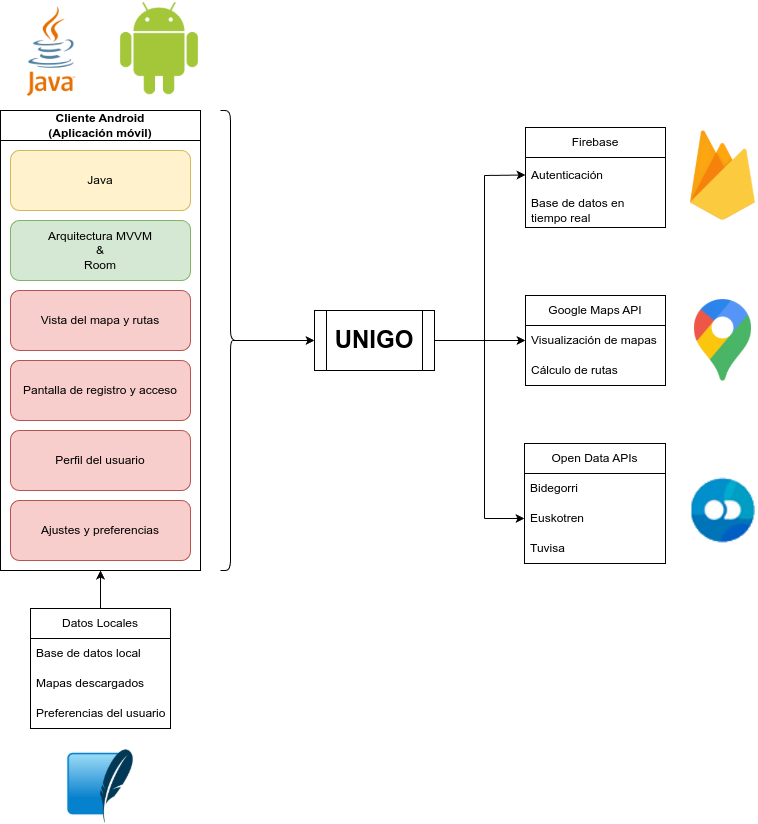
\includegraphics[width=0.7\textwidth]{../.img/arquitectura.png}
        \caption{Arquitectura de la aplicación UNIGO}
        \label{fig:arquitectura}
      \end{figure}
\end{document}